\documentclass[final,11pt,a4paper,twoside,titlepage]{article}
\input mafeuilledestyle.tex
\usepackage{graphicx}
\usepackage{url}
\usepackage[titles]{tocloft} % Control the fonts and formatting used in the table of contents.
\setlength{\cftbeforesecskip}{1ex}
\setlength{\cftsecindent}{4ex}
\setlength{\cftsecnumwidth}{6.5ex}
\setlength{\cftsubsecindent}{7ex}
\setlength{\cftsubsubsecindent}{13ex}
\setlength{\cftsubsubsecnumwidth}{4ex}

\newcommand{\p}{\vspace{0.3em}}
\newcommand{\code}[1]{\texttt{#1}}
%on utilise l'utf8 dans ce document (donc pas de \'{e} qui sont immondes...)
%je propose d'utiliser pdflatex --> illustrations en PNG



\author{Les étudiants \textbf{L3IF} du \textbf{Projet2} présentent}
\title{CoMFoRT}
\subtitle{Content Management For Teachers and Researchers}
\date{\today}
\location{Lyon}


\begin{document}
\maketitle

\abstract{
CoMFoRT est un système de gestion de contenu. Il permet aux chercheurs de créer
puis de maintenir facilement et simplement un site web agréable et bien
présenté, sans pour autant avoir à éditer des pages web directement.
La création, le remplissage et la publication du site sont autant de tâches
automatisées et agrémentées de fonctionnalités spécifiques (gestion des
publications, des enseignements).
\clearpage

\tableofcontents

\part{Vue d'ensemble du projet}
  \section{La motivation initiale~: offrir à tout chercheur un site web}
    L'idée initiale de ce projet2 nous est venue en nous promenant sur les sites
    web des chercheurs de l'ENS Lyon~: rares sont les académiciens qui
    savent mettre en valeur leur travaux personnels sur la toile. \p
    
    Beaucoup ne prennent
    pas le temps de se plonger dans les arcanes de la création d'un site web, et
    certains, peu soucieux du résultat final, copient/collent des bouts de HTML
    trouvés à droite à gauche, créant un patchwork qui n'a de site web que le
    nom. Aspect très <<~1995~>>, code source absolument terrifiant sont autant
    de raisons qui nous ont poussés à lancer ce projet.

  \subsection{Pourquoi faut-il un site web~?}
    À l'heure actuelle, la plupart de l'information circule \emph{via}
    des moyens électroniques, que ce soit des bases de papiers (ieee.org,
    acm.org) ou des moteurs de recherche (Google Scholar) dédiés au monde de la
    recherche. Le premier réflexe d'un étudiant ou d'un confrère est donc
    d'aller visiter l'organe représentatif de l'auteur dans le monde
    électronique~: son site web.\p
    
    De plus, de même qu'un chercheur, même excellent,
    fera toujours mauvaise impression s'il arrive mal habillé à une conférence,
    un mauvais site web donnera toujours un a priori négatif. En revanche, un
    site joli et simple permet à la fois de donner une bonne impression tout en
    fournissant un accès plus facile à l'information. Il nous paraît donc
    crucial pour un chercheur d'avoir un représentant <<~à la hauteur~>> sur la
     toile.

  \subsection{Pourquoi les sites actuels sont-ils aussi pauvres~?}
    Plusieurs raisons expliquent cet état de fait. Tout d'abord, le site web
    rentre souvent dans la catégorie des <<~à-côtés~>>~: il y a toujours quelque
    chose de plus intéressant à faire. La programmation web est
    souvent méprisée, considérée comme <<~de la programmation qui tache~>>.
    Pourquoi s'abaisser et passer du temps à une chose aussi futile~? \p
    
    Par ailleurs, maintenir un site web exige du temps~: il faut ajouter des
    nouvelles, mettre à jour sa bibliographie, présenter les prochains
    événements\ldots autant de tâches qui constituent une excuse pour ne mettre
    à jour le site web que quand il n'y a vraiment, vraiment rien d'autre à
    faire. \p
    
    Enfin, le concept de <<~site joli~>> est parfois difficile à saisir~: même
    un chercheur y mettant la meilleure volonté du monde n'aura pas toujours la
    fibre artistique lui permettant de créer un site web dont l'aspect sera
    agréable visuellement. \p
    
    Toutes ces raisons nous ont poussés à créer CoMFoRT~: Content Management For
    Researchers and Teachers. CoMFoRT est un logiciel d'aide à la création de
    site web~: en déchargeant le chercheur de tous les aspects sales et
    bassement techniques, ce dernier peut se concentrer uniquement sur le
    contenu. La création du site à proprement parler et l'aspect esthétique
    sont totalement pris en charge par le logiciel. Les
    chercheurs n'ont désormais plus d'excuse pour ne pas avoir un site web~!

  \subsection{Enquête de terrain auprès du public visé}
    Nous avons réalisé une enquête auprès des chercheurs et enseignants des
    différents départements de l'ENS Lyon afin de cibler les attentes du public de notre
    CMS. Il s'est dégagé un certain nombre de points sur lesquels notre
    attention a été attirée~:
    \begin{itemize}
    \item notre CMS devait permettre une gestion du site peu coûteuse en temps. La plupart des
    sondés passent en effet en moyenne une heure par mois à tenir leur site à jour.
    \item nous leur avons demandé s'ils préféraient une gestion en ligne ou en local de leur
    site et une nette majorité s'est dégagée pour une gestion en local, la version en
    ligne ne se justifiant pas selon eux.
    \item le module de news a été requis par une proportion non négligeable des gens interrogés.
    \item proposer une bibliothèque de thèmes bien fournie semble être un plus pour beaucoup
    des sondés.
    \item les opinions étaient plus partagées sur la syntaxe à utiliser~: au DMI le \LaTeX~ l'emporte
      mais dans les autres départements le wiki est plus apprécié.
    \item d'une manière globale, notre CMS devait créer facilement des pages qu'on pourrait
    ensuite facilement éditer et configurer.
    \end{itemize}
    Au cours de cette enquête nous avons pu aussi collecter l'avis de différentes
    personnes qui nous ont parfois beaucoup aidé à (ré)orienter notre projet, on notera
    ainsi l'<<~apport~>> de G.~Vidal du service Pr@tic ou les craintes maintes fois formulées que nous
    risquions de <<~réinventer la roue~>>.


  \section{État de l'art}
    \subsection{L'esprit chercheur~: KISS}
      Un point important dont nous avons pris conscience lors de la phase
      prospective, est que les chercheurs ne veulent aucune fonctionnalité
      évoluée. Les commentaires que pourraient laisser des visiteurs, des
      animations, ne présentent en général aucun intérêt pour le chercheur.
      Habitude prise à force de rédiger des pages à la main~? Toujours est-il
      que pour le chercheur, un site web est un ensemble de pages HTML, un
      ensemble de pages qui ne bouge pas. Oubliée, donc, l'idée d'un site web
      dynamique, c'est à dire qui génère la page à chaque fois qu'un visiteur la
      demande. Le site
      web du chercheur est statique~: une fois copié sur son espace web, il ne
      bouge pas, et ne change que lorsque le chercheur effectue une mise à jour.

    \subsection{Les CMS actuels~: tous dynamiques}
      Le problème est que cette logique est très spécifique~; de fait, aucun
      produit actuellement présent sur le marché ne permet de répondre à cette
      problématique.  Tous les CMS (Content Management System, Systèmes de
      Gestion de Contenu) sont dynamiques~: soutenus par une base de données
      lourde (type MySQL, le plus souvent), ils constituent un véritable
      site-portail, qui, en s'appuyant sur la base de données, extrait
      l'information à chaque fois que la page est demandée, pour la servir au
      visiteur.\p

      Pour un chercheur, un tel mode de fonctionnement est inenvisageable~: il a
      donc fallu penser notre système autrement, c'est d'ailleurs tout l'intérêt
      de CoMFoRT.

  \section{La logique de CoMFoRT}
    CoMFoRT est donc un \emph{générateur de sites}. CoMFoRT aide le
    chercheur à remplir son site. Il lui propose d'abord de choisir un thème et
    un titre. Le chercheur sera ensuite invité à ajouter du contenu~: sa
    bibliographie, ses coordonnées, les prochains événements\ldots Il 
    pourra aussi choisir quelles pages composeront son site, quel
    sera le contenu qu'il faudra mettre dans chaque page. Enfin, il saisira pour
    chaque page un texte personnalisé~: page d'accueil <<~Bonjour, bienvenue sur
    mon site\ldots~>>, et ainsi de suite.\p

    Une fois cette étape de <<~remplissage~>> du site terminée, le chercheur
    pourra \emph{générer} le site une bonne fois pour toutes~; CoMFoRT se
    chargera de l'envoyer sur son espace de stockage afin qu'il soit accessible
    par le web.\p

    La simplicité est le mot d'ordre~; CoMFoRT se veut le plus intuitif
    possible. Le chercheur n'aura donc jamais à éditer de HTML. Lorsqu'il voudra
    saisir du texte, la syntaxe sera celle de Wikipédia (une syntaxe wiki)~:
    la plupart des chercheurs sont déjà familiarisés à cet outil.

  \section{Plus de détails sur CoMFoRT}
    \subsection{Installation}
      Un installateur a été réalisé pour les systèmes Microsoft™ Windows®, à
      l'aide de NSIS (Nullsoft Installer System)~: il vérifie automatiquement les
      dépendances et la version de Python, ajoute les entrées dans le menu
      démarrer puis lance le logiciel une fois l'installation terminée.
      
      Pour ce qui est de \textsc{Linux}, un ebuild pour Gentoo a été réalisé. Un
      paquet Debian est également en cours de réalisation\footnote{Cela devrait
        normalement être terminé mais la volonté de réaliser un paquetage un minimum
        propre a entraîné des modifications profondes dans le code pour remédier à
        une importante erreur de conception d'où un retard considérable.}, ce qui
      permettra de couvrir la majorité des utilisateurs.

      Enfin, pour MacOS X, un installateur sera peut être réalisé.
      %je m'avance là non ?
      %oui, Alexandra, ça en est où ?

    \subsection{Difficultés rencontrées}
      On avait initialement stocké toutes les données du site en plein milieu du code
      ce qui empêchait toute réalisation d'une installation correcte sur un système
      multi-utilisateurs. Ceci a dû être modifié tardivement, ce qui ne s'est pas fait
      sans heurts.

    \subsection{Utilisation}
      Le code est découpé en \emph{modules} qui remplissent chacun une tâche
      particulière, et qui peuvent être paramétrés au travers de l'interface
      d'administration. Citons comme exemple de modules le module <<~News~>>, le
      module <<~Coordonnées~>>, et le module <<~Wiki~>>. Tous sont détaillés
      dans les sections qui suivent.
      
    \subsection{Considérations techniques}
      \subsubsection{Le langage utilisé}
        Nous avons utilisé Python pour réaliser ce site web. Langage élégant,
        moderne, puissant, doté d'une bibliothèque standard impressionnante,
        Python est parfaitement adapté à cette tâche. Doté d'une couche objet
        évoluée, Python permettra à tous ceux qui se sont investis dans le cours
        de Projet2 de maîtriser un langage qui leur permettra par la
        suite de réaliser facilement et rapidement des applications performantes.

      \subsubsection{Fonctionnement en détail}
        Lors de la phase de <<~remplissage~>> du site, un serveur Python est
        lancé, et c'est à l'aide d'une interface Web que le chercheur remplit son
        site. \p
        
        Cette interface web présente deux avantages~: elle est tout d'abord
        plus facile à développer qu'un client lourd (en Gtk+ par exemple), et plus
        portable. Ensuite, cette interface Web permet au chercheur d'avoir un
        aperçu <<~en temps réel~>> de son site~: en effet, cette interface locale
        (nous l'appelons la \emph{version locale}) comporte deux parties. La
        partie \emph{administration} permet au chercheur de remplir le site. La
        partie \emph{visualisation} permet au chercheur de voir après chaque
        modification à quoi ressemblera son site. Cette version locale est donc
        dynamique~: lorsque le chercheur teste son site, les pages sont générées à
        chaque fois.\p

        L'interface d'administration comporte un lien <<~synchroniser~>> qui
        permet au chercheur d'envoyer le site vers son espace Web. Là, les pages
        sont toutes générées en HTML, stockées dans un dossier, puis envoyées
        \emph{via} FTP ou SSH~: c'est la \emph{version statique}. Naturellement,
        l'interface d'administration n'est pas générée ou envoyée sur l'espace
        Web~; l'interface d'administration n'existe que dans la version locale.

      \subsubsection{Utilisation alternative~: en CGI avec Apache}
        Il est à noter qu'une utilisation alternative, bien que fortement
        déconseillée, est possible. Plutôt que d'utiliser le serveur en Python livré
        avec CoMFoRT pour faire tourner la version locale, il est possible de la
        faire tourner dans le serveur Apache. C'est une utilisation totalement à
        contre-emploi de CoMFoRT~; elle reste néanmoins possible. Il appartient
        alors à l'utilisateur de s'assurer que sa partie administration est
        correctement protégée à l'aide de fichiers \code{.htaccess}.


\part{La gestion de contenu}
  \section{La partie administration (WP1)}
    \subsection{Objectif~: simple et efficace}
      Le rôle de la partie administration est de permettre à
      l'utilisateur de gérer de manière efficace le contenu de son site. Cette
      partie de CoMFoRT est donc primordiale et doit être réfléchie pour être
      intuitive et facile d'accès. Elle se décompose en trois parties~: la 
      configuration générale, la configuration des modules et la génération du 
      site.
      
      \vspace{1em}
      \begin{center}
      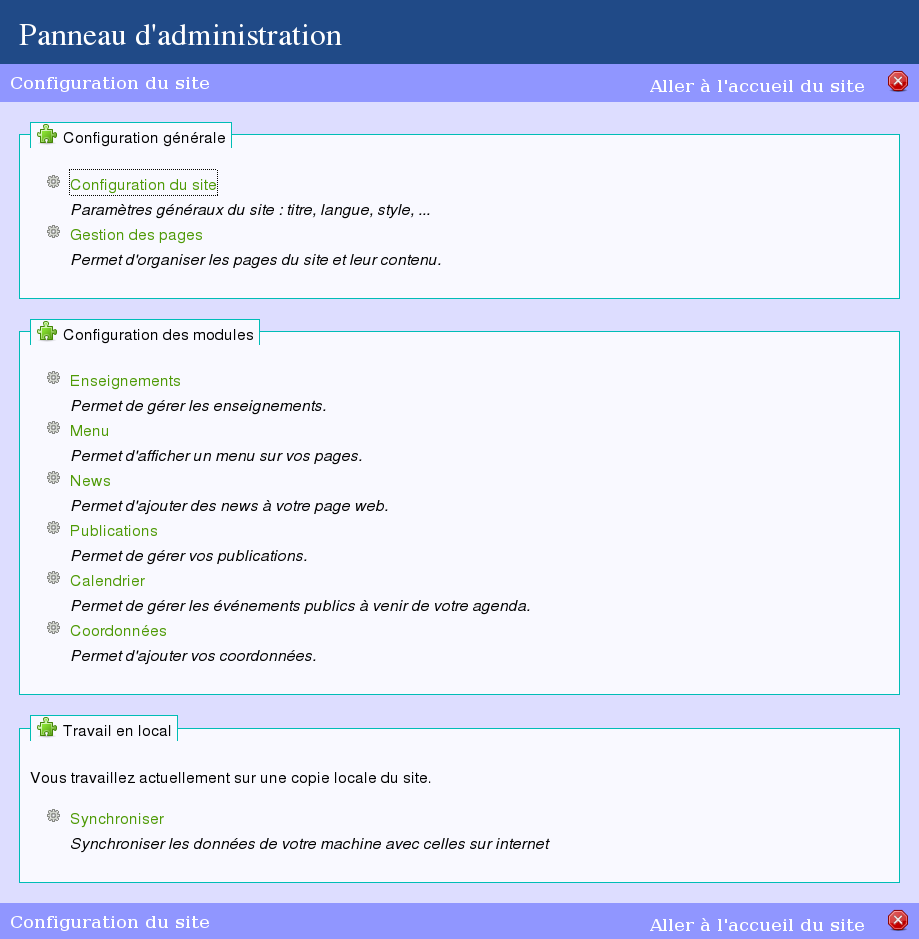
\includegraphics[width=16cm]{admin_general.png}
      \end{center}
      \vspace{1em}
      
      \begin{itemize}
      \item \emph{Configuration générale~:}
        Cette partie de l'administration permet de gérer la structure générale 
        du site~: son titre, sa langue par défaut (pour l'instant, cela concerne
        uniquement la langue de l'administration), le style CSS utilisé et 
        surtout l'ensemble des pages du site et leur contenu.
      
        La gestion des pages consiste principalement à ajouter/supprimer des
        pages, à choisir les modules actifs sur telle ou telle page ainsi que
        leur ordre d'affichage et à modifier le contenu de la page via le wiki.
        \p
      
      \item \emph{Configuration des modules~:}
        Chaque module (autre que le wiki) possède sa propre page de 
        configuration, ce qui fait que CoMFoRT est facile à configurer et à
        prendre en main.
        De plus, cette partie a été pensée pour faciliter la vie à des
        développeurs éventuels. En cas d'ajout d'un module, l'administration se 
        met automatiquement à jour~: elle propose un lien pour configurer le 
        nouveau module et modifie la base de données pour tenir compte de
        celui-ci.\p
      
      \item \emph{Génération du site~:}
        Cette partie de l'administration gère les paramètres relatifs à la
        connexion FTP ou SSH et permet de publier le site sur internet en un
        seul clic.
      \end{itemize}
      
    \subsection{Moyens mis en oeuvre}
    Les formulaires de l'interface ne sont pas statiques et dépendent du contenu
    de la base de données. Il est donc nécessaire de les générer. Or, à la 
    différence du PHP, le Python ne peut pas s'insérer dans du XHTML et il est
    alors nécessaire de générer entièrement la page demandée par l'utilisateur.
    \p
    
    Pour faciliter le travail d'implémentation et la lisibilité du code, nous
    avons développé une classe qui gère les balises XHTML, leurs attributs et
    leur contenu ce qui permet de produire facilement du code XHTML 1.0 
    Transitionnel valide (il n'y a pas de problème de balises mal imbriquées ou
    mal appareillées, d'attribut sans guillemets, etc\ldots).\p
    
    Enfin, il s'agit aussi de récupérer les données des formulaires. Il faut
    vérifier les données entrées et signaler une erreur le cas échéant.
    Elles sont ensuite stockées, dans un fichier ou dans la base de données
    selon leur nature.\p
      
    \subsection{Stockage des données}
    Toutes les données concernant les pages du site sont stockées dans la base
    de données. 
    Les autres paramètres sont stockés dans l'un des fichiers suivants, dans le
    répertoire \code{.comfort} de l'utilisateur~:\p
    \begin{itemize}
    \item \code{conf\_private.py}~: Les paramètres relatifs au transfert FTP ou
    SSH.
    Notons que le mot de passe FTP n'est pas stocké~: il est redemandé à chaque
    synchronisation pour être envoyé directement au serveur. L'utilisateur est
    libre d'utiliser le gestionnaire de mot de passe de son navigateur s'il ne
    souhaite pas ressaisir le mot de passe à chaque fois.\p
    
    \item \code{conf\_general.py}~: Ici sont stockés le titre, la langue, les 
    styles pour l'admin et le site, etc\ldots. Il est plus que conseillé de ne
    pas le modifier. Remarquons cependant la présence d'une variable
    \code{display\_logo}. Pour afficher l'encombrant logo de CoMFoRT en bas de
    page, il suffit de la passer à 1.
    \end{itemize}
    
    \subsection{Difficultés rencontrées}
      L'administration reflète donc toutes les possibilités offertes à 
      l'utilisateur ce qui en fait la partie émergée du projet. C'est pour cette
      raison que l'évolution de l'administration est intimement liée à
      l'évolution du projet: il fallut fournir un travail constant tout le long
      du développement pour l'adapter aux changements de cap et aux nouvelles
      fonctionnalités. \p
      
      Ainsi, nous avions initialement prévu de proposer la possibilité d'éditer
      le site en ligne. Il y avait donc une partie de l'administration pour
      gérer le mot de passe pour sécuriser la gestion "online" du site. Cette
      partie a finalement été supprimée car l'édition en ligne ne fait plus
      partie des objectifs de CoMFoRT. Nous avons ensuite du procéder à une
      restructuration
      des formulaires à cause du découpage en modules~: il a été décidé qu'ils
      géraient eux-mêmes leurs formulaires de configuration. Il a aussi fallu
      intégrer le wiki assez tardivement, lorsque les possibilités de celui-ci
      ont été définies avec certitude. Parallèlement, l'évolution 
      régulière de la nature des données à stocker et de la manière
      de le faire nous a aussi obligé à patcher régulièrement la validation des
      formulaires. Enfin, il a fallu trouver un style agréable et convivial pour
      l'administration, ce qui est important pour l'ergonomie du projet.


  
  
  \section{Les modules (WP4 et 5)}
  
%  \vspace{0.5cm}

    
    Nous avons conçu pour le logiciel une architecture modulaire qui essaye de
    tirer au mieux parti des fonctionnalités objet de Python.\p

    \begin{center}
      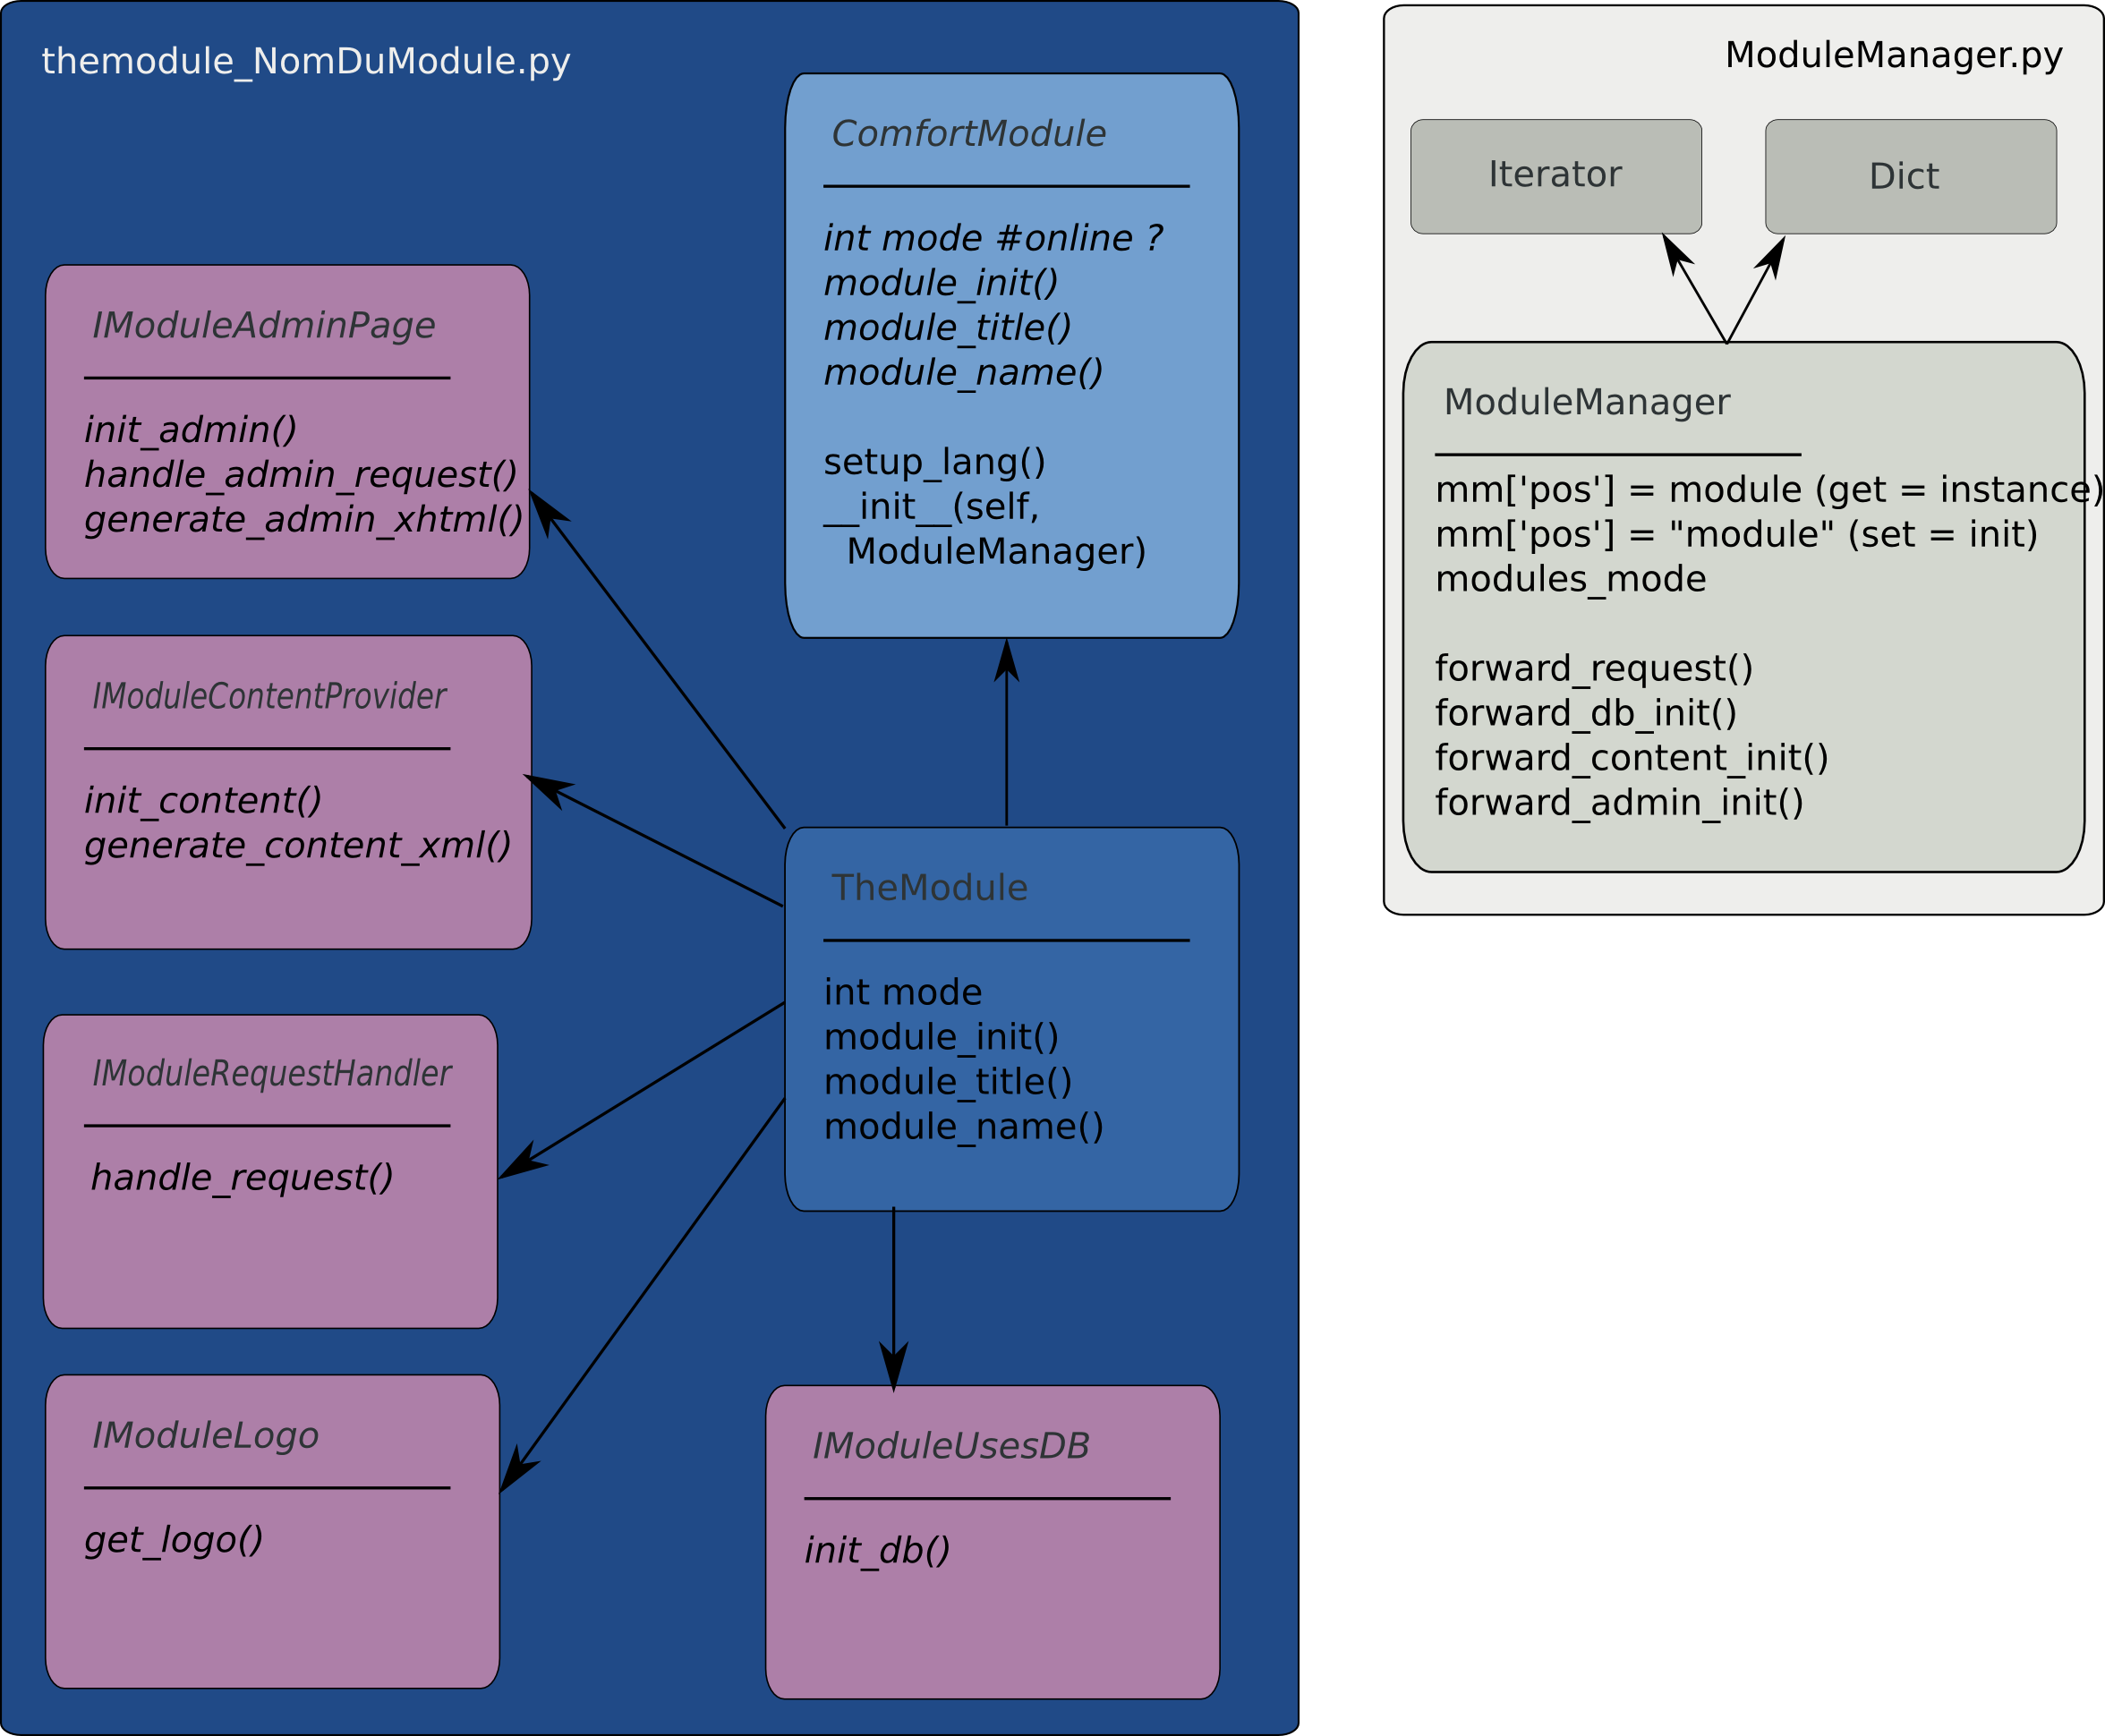
\includegraphics[width=16cm]{rect3581.png}
    \end{center}

    Chaque module implémente une interface selon les fonctionnalités qu'il
    propose~: \code{IModuleAdminPage} pour les modules ayant une page dans le
    panneau d'administration, \code{IModuleContentProvider} pour les modules
    générant du contenu, \code{IModuleUsesDB} pour les modules utilisant la base
    de données\ldots d'autres interfaces ont été prévues mais pas encore
    utilisées~: elles le seront dans une prochaine version.\p

    Ainsi, si l'on veut écrire un module, il suffit de créer un fichier
    \code{themodule\_NomDuModule.py} et d'écrire une classe implémentant les
    interfaces voulues, selon ce que fait le module.\p
    
    Le \code{ModuleManager} est la classe qui se charge de gérer
    l'initialisation d'un module, le fait de propager la langue utilisée à
    chaque module, de propager l'objet de la base de données à chaque module qui
    en a besoin, et ainsi de suite. Elle implémente le \emph{Design Pattern}
    singleton. Elle profite encore un fois au mieux des fonctionnalités de
    Python, puisqu'on peut l'utiliser comme un dictionnaire ou comme un
    itérateur. Python montre encore une fois ses avantages, en nous offrant une
    syntaxe claire et performante.\p

    Le \code{ModuleManager} est le squelette de CoMFoRT~: c'est l'un des
    premiers éléments de la page à être initialisés, et c'est lui qui fait le
    lien entre les différents modules.



  \section{Le module Wiki}
    \subsection{Pour éditer le contenu de vos pages~: le wiki}
      Pour ajouter à vos pages des éléments que ne proposent pas les autres
      modules, plus besoin d'éditer vos pages à la main comme au bon vieux
      temps. Le wiki est là pour vous simplifier la vie. Il a tout d'un grand et
      reprend une grande partie de la syntaxe largement répandue de Wikipédia.
      Il permet entre autres de
      formater le texte et d'insérer titres, lien hypertextes, images, tableaux,
      listes et références en toute simplicité.\p

      Soucieux de servir l'intérêt des chercheurs, nous avons aussi ajouté la
      possibilité d'insérer des formules \LaTeX{}. Il suffit pour cela
      d'utiliser la balise \code{<math size="200" packages="paquet1
      paquet2\ldots">formule LaTeX ici </math>}.
      La formule sera alors automatiquement convertie en image grâce à
      \code{l2p} (un logiciel de Aaron Maxwell) puis insérée dans la page.
      L'attribut
      \code{size} permet de régler la taille de l'image produite et
      \code{packages} permet de spécifier les paquets nécessaires à \LaTeX{}
      pour générer la formule.

    \subsection{Un module un peu spécial}
      Le wiki génère par essence un contenu propre à chaque page ce qui le rend
      différent des autres modules, dont le contenu ne varie pas entre les pages
      . De fait, son interface a été intégrée à l'interface de gestion des pages
      . Celle-ci s'inspire encore une fois de Wikipédia en reprenant les boutons
      qui permettent d'insérer facilement du code wiki. Mais elle apporte aussi
      une fonctionnalité CoMFoRTable~: il est possible d'insérer en un seul clic
      des liens vers les pages du site et pages, images et documents personnels.
      
      \vspace{1em}
      \begin{center}
      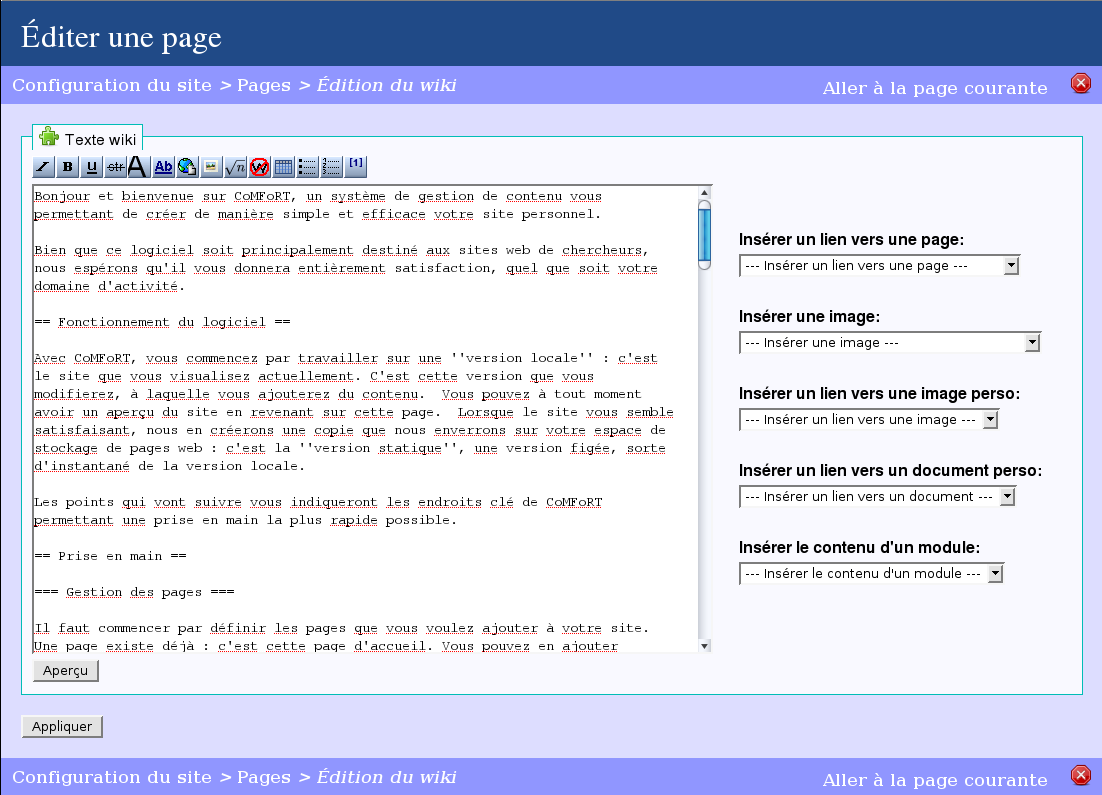
\includegraphics[width=16cm]{admin_wiki.png}
      \end{center}
      \vspace{1em}

      Toutes ces fonctionnalités vous permettent de créer des pages claires et
      structurées facilement et rapidement tout en garantissant un code
      \emph{XHTML 1.0 Transitional} fiable et lisible.

    \subsection{Fonctionnalité avancée}
      Pour rendre le Wiki encore plus flexible, nous lui avons ajouté un dernier
      atout. Il est possible d'insérer un module à l'intérieur même du Wiki
      grâce à la balise
      \begin{center}
      \code{<module id="moduleID" params="paramètres" />}.
      \end{center}
      Cela se fait facilement grâce à une liste des modules disponibles.\p

      Le premier avantage de cette balise est de lever la restriction sur
      l'enchaînement linéaire des modules~: sans cette balise, il n'était par
      exemple pas possible de créer une page avec du wiki avant et après le
      module Publications.\p

      Outre cette amélioration déjà non négligeable, la balise \code{<module>}
      augmente aussi grandement les possibilités pour gérer le contenu du site.
      Le champ \code{params} de la balise permet de passer des paramètres en
      argument au module sous la forme
      \begin{center}
      \code{paramètre1=valeur1\&paramètre2=valeur2\&\ldots}
      \end{center}\p

      Le module \emph{Publication} utilise par exemple cette fonctionnalité pour
      afficher un contenu différent suivant les arguments.\p

      Le module Wiki est donc un module essentiel de CoMFoRT~: ses
      fonctionnalités basiques en font un outil efficace pour éditer vos pages
      et son utilisation avancée offre des possibilités multiples ainsi qu'une
      grande flexibilité.

  \subsection{Difficultés rencontrées}
    La tâche du module Wiki est principalement d'analyser le code wiki entré par
    l'utilisateur et de le transformer en DocBook. Cette opération est
    normalement assez simple, à condition d'avoir à sa disposition la grammaire
    décrivant la syntaxe wiki.\p
    
    Ce n'était cependant pas le cas ici: nous avons cherché cette grammaire, 
    sans succès. Il a donc fallu la recréer. En voici le détail:
    
    \begin{verbatim}  
tokens :=  <EOF> | <return> | <string> |
           <"="> | ... | <"======"> |
           <"''"> | <"'''"> |
           <"|"> | <"["> | <"]"> | <"[["> | <"]]"> | <"{{"> | <"}}"> |
           <"{|"> | <"|}"> | <"|+"> | <"|-"> | <"!"> |
           <":"> | <"#"> | <"*"> | <blank> | (en début de ligne)
           et toutes les balises
           
          
wiki  := { wiki_content } <EOF>

wiki_content :=   titre 
                | paragraphe 
                | code 
                | structure
                | tableau
                | balise_simple 
                | balise_double 
                | <return>
  
titre :=   <"=="> texte <"=="> 
         | <"==="> texte <"===">
         | <"===="> texte <"====">
         | <"====="> texte <"=====">
         | <"======"> texte <"======">
       
paragraphe := texte { [ <return> ] texte }
           
texte := ligne { ligne }
  
ligne :=  contenu <return>
  
contenu := { <string> | format | lien | exposant_indice }
       
format :=   <"''"> contenu <"''">
          | <"'''"> contenu <"'''">
            
lien := lien_interne | lien_externe | image
  
lien_interne := <"[["> [ type_lien ] <string> [ <"|"> <string> ] <"]]">
                                    
type_lien := "Picture:" | "Page:" | "Doc:"
  
lien_externe := <"["> <string> [ <"|"> <string> ] <"]">
  
image := <"["> "Image:" <string> options <"]">
                                 
options := [ <"|"> "thumb" ] [ <"|"> position ] [ <"|"> size ] [ <"|"> <string> ]
 
position :=   "left" 
            | "center" 
            | "right"
  
size :=   <number> "px" 
        | <number> "x" <number> "px"
        | <number>
          
exposant_indice :=   <"{{"> texte <"}}">
                   | <"{{"> "ind" <"|"> texte <"}}">
                   | <"{{"> "exp" <"|"> texte <"}}">
          
code := <blank> ligne { <blank> ligne }      
  
structure := ( <":"> ligne ) | 
             ( ( <"#"> | <"*"> ) struct_rec )
  
struct_rec := paragraphe | structure
  
balise_simple :=  "<br />" | "<br>"
                  "<hr />" | "<hr />"
                  "<module" params ( "/>" | ">" )                
  
balise_double :=   "<h2>" contenu "</h2>"
                 | "<h3>" contenu "</h3>"
                 | "<h4>" contenu "</h4>"
                 | "<h5>" contenu "</h5>"
                 | "<h6>" contenu "</h6>"
                 | "<math" params ">" <preformated_string> "</math>"
                 | "<nowiki>" <preformated_string> "</nowiki>"
                 | "<pre>" <preformated_string> "</pre>"
                 | "<center>" texte "</center>"                       
                 | "<s>" texte "</s>"
                 | "<u>" texte "</u>"
                 | "<b>" texte "</b>"
                 | "<i>" texte "</i>"
                 | "<highlight>" texte "</highlight>"
                 | "<big>" texte "</big>"
                 | "<small>" texte "</small>"
                 | "<sub>" texte "</sub>"
                 | "<sup>" texte "</sup>"
                 | "<ul>" texte "</ul>"
                 | "<ol>" texte "</ol>"
                 | "<li>" texte "</li>"
                 | "<ref>" texte "</ref>"                 

params := { { " " } <string> "='" <string> "'" }

tableau := <"{|"> [tableau_titre] tableau_contenu <"|}">

tableau_titre := <"|+"> texte

tableau_contenu := { <"|-"> | tableau_ligne_contenu }

tableau_ligne_contenu := (<"|"> | <"!">) [ tableau_cellule_option <"|"> ] texte

tableau_cellule_option := ( "align=" ( "left" | "center" | "right" ) ) |
                          ( "valign=" ( "top" | "middle" | "bottom" ) ) |
                          ( "colspan=" <number> ) |
                          ( "rowspan=" <number> )
                                                   
  \end{verbatim}

  \section{Le module Calendrier}
    Annoncer ses publications imminentes, donner la date de sa prochaine intervention,
    c'est-à-dire publier son calendrier est l'une des fonctions pour un chercheur de 
    son site web. Ce module est là pour lui permettre de le faire.\p 

    Puisque notre CMS n'est pas dynamique, il n'est pas possible de moduler l'affichage
    en fonction de la date. Néanmoins, sur demande à chaque synchronisation,
	les évènements passés peuvent être effacés et les évènements lointains non annoncés 
    afin de ne pas surcharger l'affichage.\p

    De plus, la réelle valeur ajoutée de ce module est la possibilité d'importer des
    fichiers \emph{vcalendars}. En effet, notre but étant de minimiser le travail à 
    fournir par le chercheur pour avoir un site web élégant et complet, il nous faut 
    absolument éviter de lui demander de faire des choses en double. Si lui ou son 
    équipe tient un calendrier public sous Sunbird, iCal ou Google Calendar~, il doit
    pouvoir importer directement ce fichier et n'avoir plus qu'à choisir les évènements
    qu'il souhaite voir apparaître sur sa page.

  \section{Le module Coordonnées}
    On les retrouve sur tous les sites de chercheur~: les traditionnelles coordonnées.
    Ce module permet de gérer ce qu'on appelle des jeux de coordonnées. Chacun de ces 
    jeux peut contenir un grand nombre d'informations telles que l'adresse du lieu de
    travail, plusieurs numéros de téléphone, le laboratoire, un email, ou bien encore
    un fax.\p

    L'administration du module permet d'ajouter autant de ces jeux de coordonnées que
    l'utilisateur le désire, de les éditer, de les supprimer, de manière extrêmement
    simple. \p

    Il a été également remarqué que beaucoup de chercheurs veulent afficher leurs 
    coordonnées d'une certaine manière, par exemple, les coordonnées personnelles et
    professionnelles l'une à côté de l'autre. Il y a donc deux affichages possibles.
    Soit le chercheur active le module Coordonnées sur une page, et dans ce cas, seul le 
    premier jeu de coordonnées sera affiché là où le module est activé. Soit le chercheur
    n'active pas le module Coordonnées, mais utilise le module Wiki. Comme on l'a vu, 
	il suffit d'insérer la balise \code{<module id="Coord" params="coord\_id=0" />} pour
    passer l'argument \code{coord\_id} au module~: celui-ci affichera alors le jeu de
    coordonnées de numéro \code{coord\_id}. Ainsi, on pourra mettre en forme ces jeux,
    typiquement en les insérant dans un tableau wiki à deux colonnes et une seule 
    ligne.

  \section{Le module Éducation}
    Qui dit site web de chercheurs et d'enseignants dit nécessairement module 
	d'enseignement. C'est en général une grande partie du contenu des sites et il
    était donc indispensable d'en permettre une gestion poussée mais simple et
    d'offrir un affichage automatisé mais aussi flexible. 
 
    \subsection{Interface de gestion des enseignements}
    Le module Enseignements possède une interface d'administration intuitive et 
    très facile à utiliser. En trois clics, un enseignement est créé. On notera la
    possibilité de choisir entre TD et Cours ainsi que celle de sélectionner son 
	université ou son école parmi celles déjà existantes ou nouvellement ajoutées
	(toutes les écoles entrées sont gardées dans la base de données pour pouvoir 
	les réutiliser rapidement).\p
    
    Il y a ensuite la possibilité d'ajouter des documents, que ce soient des PDF
    ou tout autre format, agrémentés de commentaires~; utile pour ajouter les
    énoncés de TD ainsi que leurs corrigés. \p

    Enfin, on pourra, grâce au module Publications, s'il existe, ajouter une 
    bibliographie à chaque enseignement. Nous espérons ainsi capter toutes les
    données nécessaires à la bonne description d'un enseignement.

    \subsection{L'affichage~: problèmes\dots}
    Un problème de taille s'est posé lors de la conception de ce module~:
    permettre un affichage flexible des enseignements. Nous avons en effet remarqué
    que beaucoup de manières différentes d'afficher les enseignements étaient 
    utilisées parmi les enseignants. Comment permettre un affichage automatique,
    avec très peu d'intervention humaine, tout en laissant un minimum de choix à
    l'utilisateur quant à l'aspect de sa page~?\p

    Impossible de permettre à l'utilisateur de placer sur sa page chaque élément,
    ce serait l'échec du CMS. Impossible également de ne proposer qu'un affichage
    linéaire des différents enseignements, car l'utilisateur se sentirait enfermé
    dans un certain schéma, sans pouvoir personnaliser sa page web.\p

    \subsection{L'affichage~: \ldots et solutions}
    La solution intermédiaire choisie lors de la conception de ce module est la 
    suivante~: l'affichage par défaut, choisi lorsque l'on active le module sur
    une page est l'affichage linéaire, élégant mais prenant beaucoup de place si
    beaucoup d'enseignements sont présents. Cependant, il est possible de cliquer
    sur le bouton <<~Affichages spéciaux~>> pour arriver sur un formulaire proposant
    différents modes d'affichage. Cette fonctionnalité n'est présente que si le
    module wiki est activé et elle en utilise au mieux les caractéristiques.
    En fait, le module va générer toutes les pages (elles apparaissent donc dans
    le formulaire de gestion des Pages) avec le code wiki (en général, simplement 
    une balise module avec avec les arguments corrects) nécessaire à l'affichage
    demandé. Le module fournit ensuite le code wiki à insérer pour faire marcher
    le tout.\p

    Un exemple d'affichage~: on peut voir le sommaire ainsi qu'une
    partie de la page sur laquelle on arrive quand on clique sur <<~ASR~>>.

    \begin{figure}[htbp]
      \centering
      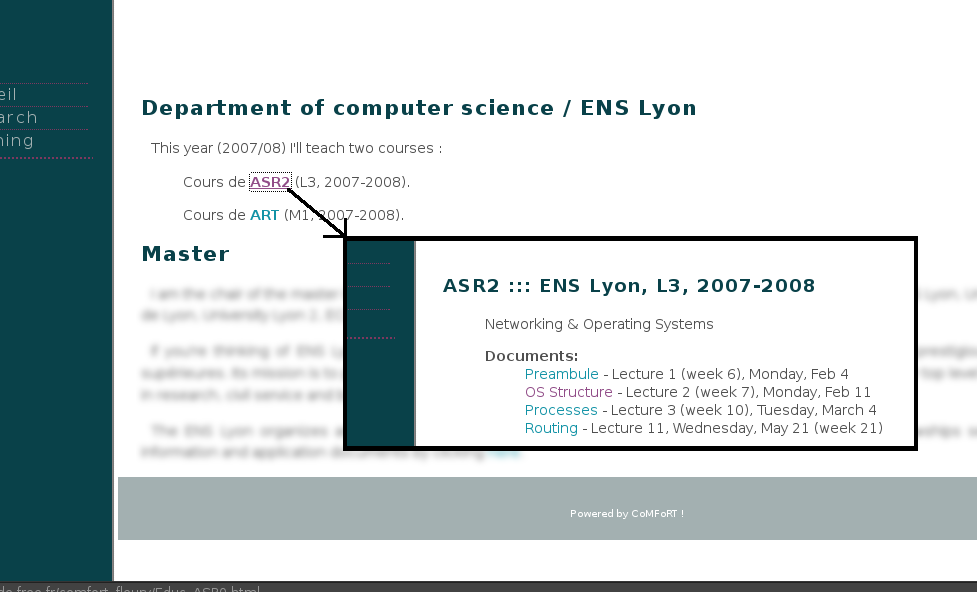
\includegraphics[width=16cm]{display_educ.png}
      \caption{\footnotesize Exemple de résultat de l'affichage type <<~short~>> du module Educ}
    \end{figure}
    
  \section{Le module Menu}
    Impossible d'avoir un site sans menu pour le structurer. Le module Menu,
    incontournable et présent par défaut sur toute nouvelle page créée, répond à
    cette nécessité. \p

    L'administration permet de d'insérer des éléments au menu de façon intuitive~: il
    suffit de donner un nom au nouvel élément (celui qui apparaîtra dans le menu) et
    de choisir dans une liste la page du site vers laquelle il renvoie. Cette liste
    de pages inclut bien sûr la liste des pages générées par CoMFoRT mais aussi les
    pages du dossier \code{perso/pages}. \p

    Toujours dans le but de faire gagner du temps à l'utilisateur,
    il est possible d'ajouter automatiquement un bouton au
    menu lors de la création d'une page, par un simple clic. De même, lors de la
    suppression d'une page, les éléments du menu qui pointaient vers cette page sont
    automatiquement supprimés.

  \section{Le module News}
    Le module News est un module très simple permettant d'ajouter très facilement
    dans une page des informations, datées, correspondant à ce que l'on appelle
    communément des news.  \p
    
    L'administration est extrêmement simple et sobre, ce module étant lui-même 
    fait pour être simple. On peut facilement ajouter, supprimer, éditer les
    news entrées dans la base de donnée. Un effort a été fait pour intégrer au
    mieux ces news dans les feuilles de style CSS, par exemple en les fondants
    dans la page.
    
  \section{Le module Publications}
    \subsection{Pourquoi~?}
    La gestion des publications, plus encore que le module Enseignements, est
    la fonctionnalité qui va de la manière la plus flagrante différencier un 
    CMS lambda et CoMFoRT, un CMS à destination des chercheurs et enseignants.
    La première phase de développement a consisté en la prise en charge du 
    format BiBTeX, format de plus en plus répandu au sein de la communauté
    scientifique. Cette prise en charge consiste en l'importation/exportation
    de fichiers BiBTeX, pour que les chercheurs puissent gérer toutes leurs 
    publications depuis CoMFoRT, ce qui est plus encore que de l'utiliser pour
    leur site web. \p

    Nous espérons également que si notre CMS se répand chez une part significative
    des chercheurs, il aide à l'uniformisation des standards de gestion de 
    publications, et qu'ainsi il participe au développement des moyens d'échange
    entre chercheurs (ne rêvons pas). On pourra penser notamment à un certain 
    nombre de chercheurs en sciences humaines (pour ne pas dire quasiment tous),
    qui ne disposent d'aucun moyen d'échanger simplement leurs bibliographies,
    listes de publications, car ils ne connaissent pas BiBTeX, plus largement
    répandu chez les scientifiques utilisant \LaTeX{}. On peut rêver et imaginer
    que cela aide à répandre BiBTeX dans cette communauté. \p

    La deuxième phase de développement a été de trouver des moyens astucieux 
    de gérer ces publications, de les regrouper par listes, de trouver un 
    moyen simple pour l'utilisateur de les afficher où il le veut, et de manière
    flexible sans être trop laxiste. Cette phase de développement a amené à 
    repenser la gestion des modules et à la balise \code{<module>} du Wiki. \p

    La troisième phase, a consisté à faire fonctionner d'autres modules avec le
    module Publications, comme par exemple le module Enseignements qui utilise
    également des bibliographies. De plus nous cherchons à rendre plus agréable
    l'utilisation de ce module et à en étendre les fonctionnalités par la prise
    en charge de plus de champs du format BiBTeX, etc\dots

    \subsection{Import/Export BiBTeX}
    Comme on l'a dit, la prise en charge du format BiBTeX est la fonctionnalité 
    essentielle du module Publications. 

    Ainsi, il est possible de faire deux choses~:
    \begin{itemize}
      \item Importer un fichier BiBTeX via l'administration. Le module va ensuite
	    parser ce fichier et ajouter à la base toutes les publications qu'il y a trouvé.
	    Pour le moment, on ne peut choisir lesquelles parmi ces publications on veut 
	    garder. Elles le sont pour l'instant toutes, mais cela fait partie
	    des améliorations à venir très rapidement.\p
  
      \item Exporter des publications au format BiBTeX. Après avoir utilisé le système
	    de listes de publications que l'on évoquera plus tard, on peut décider d'exporter
	    ces publications. Simplement en appuyant sur un bouton, on découvre avec joie un
	    fichier BiBTeX respectant parfaitement les standards. Quelques commentaires 
	    annotent ce fichier. 
    \end{itemize}

    \subsection{Importation Google}
    Un autre mécanisme d'importation, encore en cours de test et de développement (donc 
    toujours non pleinement fonctionnel) a été imaginé et implémenté~: l'importation
    de publications via Google Scholar. Pour l'utiliser, il faut bien sûr être connecté
    à Internet. Pour l'instant il se contente d'aller chercher les publications
    correspondant au nom fourni dans le formulaire. Mais à terme, il
    permettra d'afficher les 10 premières publications trouvées sur
    Google, de laisser le choix de celles que l'on souhaite garder,
    voire ajouter à une liste de publication, et celles que l'on
    rejette. Puis, on pourra passer aux 10 suivantes, et ainsi de
    suite. Cela permettrait entre autres de récupérer une bonne partie
    de sa propre bibliographie, au format BiBTeX, si l'on en dispose pas
    (on pense ici à certains chercheurs en sciences humaines qui ne
    disposent pas encore de site, et encore moins de liste de
    publications autre que manuscrite, et de fait, pas non plus au
    format BiBTeX).

    \subsection{Listes de publications}
    Une fonctionnalité extrêmement utile de ce module, et celle qui fait d'ailleurs
    tout marcher, c'est la gestion de listes de publications. Qu'est-ce donc~? 
    Simplement la possibilité de répartir les différentes publications entrées dans
    la base de donnée, à la main ou via des fichiers BiBTeX, dans différentes listes,
    pour pouvoir les gérer plus facilement. Ainsi on créera une liste "Mes publications",
    une liste "Bibliographie Cours 1", "Bibliographie Cours 2", "Transparents", ou encore
    "Conférences internationales", et on pourra afficher l'une ou l'autre via la balise
    \code{<module>} du module Wiki. Par défaut, si l'on ne fait qu'activer le module
    Publications, il affichera TOUTES les publications entrées dans la base de données,
    ce qui peut convenir si on ne fait rien de compliqué avec ses publications.

    \subsection{Problèmes rencontrés}
    Nous avons rencontré un certain nombre de problèmes liés à la gestion des publications. \p
    
    Tout d'abord, il est extrêmement compliqué, au vu des nombreuses présentations et 
    utilisations différentes des chercheurs de leurs publications sur leur site, d'imaginer
    un dénominateur commun, une gestion qui permette au plus grand nombre d'utiliser ce 
    module comme ils l'aimeraient, et qui soit à la fois très simple d'utilisation. La 
    solution imaginée a été les listes de publications, simples d'emploi et répondant
    à la plupart des besoins. Néanmoins, il reste encore beaucoup à faire sur ce point,
    et c'est ce que nous devrons améliorer lors du développement futur. \p

    Le fait que le site soit destiné à être statique nous posait un problème. En effet,
    lorsque l'on activait le module Publications sur une page, celui-ci affichait donc
    toujours la même chose, au même endroit, défini par les priorités de module. Comment
    donc faire pour que l'affichage ne consiste pas en l'affichage de toutes les listes
    de publication, les unes à la suite des autres. Comment permettre à l'utilisateur
    d'afficher plutôt une liste triée par année, par titre, etc\dots~? Il fallait pouvoir
    passer des paramètres à la fonction de génération DocBook du module. Nous avons
    donc d'abord penser à récupérer en local (sur le serveur faisant marcher python)
    les arguments passés via la méthode GET, c'est-à-dire du type~: 
    \code{handler.py?page=publis.html\&arg1=val1\&arg2=val2}\dots Puis,
    lors de la synchronisation, nous aurions généré des pages
    correspondant à chaque valeur des arguments, et modifié
    en conséquence les liens. Néanmoins, c'était lourd et inefficace. 
    Nous avons donc finalement opté pour une modification du module Wiki, en insérant la
    balise \code{<module>}. Ainsi, le problème de l'affichage flexible des listes de 
    publications est réglé, et cela a permis aux autres modules de s'affranchir du côté
    trop statique imposé par la gestion initiale des modules.
  
  \section{Le dossier personnel}
    Pour permettre d'ajouter à votre site des éléments plus personnels, une
    solution existe: le dossier \code{$\sim$/.comfort/perso}.\p    
    
    \begin{itemize}
      \item Vous pouvez rajouter des pages personnelles à votre site, ou même
        des modules externes à CoMFoRT (un module de photos en PHP par exemple).
        Ajoutez vos pages dans \emph{$\sim$/.comfort/perso/pages} et elles seront
        directement accessibles depuis le menu ou le wiki (voir ci-dessous).\p
      \item Il est également possible de rajouter des images
        (par exemple une photo personnelle) dans 
        \emph{$\sim$/.comfort/perso/pictures}. Encore une fois, vous y aurez accès
        grâce au module wiki. \p
      \item Il en est de même pour toutes sortes de documents que vous souhaitez
        rendre accessibles: il suffit de les placer dans 
        \emph{$\sim$/.comfort/perso/docs}. Notons toutefois que le module
        Enseignement modifie ce dossier en y ajoutant tous les documents
        relatifs aux enseignements que vous avez créés et en les renommant.
        Il est alors possible de faire une mise à jour de ces documents 
        simplement en écrasant l'ancienne version manuellement (les nouveaux 
        noms après renommage sont disponibles dans le module Enseignement)
    \end{itemize}    \p
    Il vous est possible de modifier librement le contenu de ces répertoires
    et de créer des sous-répertoires pour les organiser comme bon vous semble.
    Lors de la génération du site, cette organisation sera conservée.

  \section{La localisation et l'internationalisation (WP7)}

    \subsection{Les langues et CoMFoRT}
    Logiciel éloboré par des étudiants français, CoMFoRT est disponible
    en français. Cependant, bien que les résultats de l'enquête
    préliminaire soient fondés sur des chercheurs français, le public
    visé doit être élargi aux chercheurs et enseignants du monde
    entier. Modestement, CoMFoRT n'a pour l'instant été rendu disponible
    qu'en anglais. C'est à dire qu'il est possible d'avoir le logiciel
    (menu, options de configuration) en anglais ou en français, et la
    documentation utilisateur est disponible dans ces deux langues. La
    traduction du logiciel en d'autres langues est facilitée par l'utilisation
    de l'outil GNU/gettext.

    \subsection{Gettext}
    GNU/gettext est un logiciel libre qui vise à permettre une meilleure
    adaptation des logiciels aux utilisateurs. La plupart des logiciels
    sont écrits en anglais, que ce soit parce que l'équipe de
    développement est américaine, ou parce que c'est la principale langue
    commune aux différents contributeurs, ou encore parce que c'est de cette
    manière que le public visé par le produit sera le plus
    large. Cependant de nombreuses personnes ne sont pas capables de
    comprendre parfaitement l'anglais, il faudrait donc des versions
    adaptées des logiciels pour ces personnes. Gettext automatise la
    création de ces différentes versions. Sans réelle contrainte pour
    les programmeurs, il est possible de faire générer à gettext des
    fichiers de localisation. Ces fichiers contiennent la liste des
    chaînes de caractères à rendre disponibles en plusieurs langues. Un
    traducteur édite ensuite ces fichiers pour ajouter les phrases
    équivalentes dans la nouvelle langue. Finalement lors de
    l'utilisation du logiciel, suivant la configuration choisie ou les
    paramètres par défaut de l'environnement, la version linguistique
    est définie.

    Dans la version actuelle de CoMFoRT, les chaînes de caractères sont
    pour l'instant écrites en Français dans le code, et seront donc à
    traduire du français vers la langue souhaitée par les
    contributeurs. À terme elles seront remplacées par leurs équivalents
    en anglais pour faciliter l'ouverture à d'autres horizons linguistiques.
    
    \subsection{Module International}

    Force est de constater que nombreux sont les chercheurs qui proposent
    leur site en plusieurs langues. L'idée d'offrir un module facilitant
    ce travail est alors naturelle. Il s'agirait d'associer à chaque
    page créée une langue, et de proposer d'associer les pages sur le
    même sujet en différentes langues. Ainsi il serait possible d'avoir
    un menu unifié, avec les liens du menu pointant vers des pages de
    même langue. Un bouton ou un lien permettrait de passer d'une langue
    à une autre. Les pages non disponibles dans la langue actuelle
    pourraient ne pas apparaître dans le menu, ou alors apparaître dans
    une langue par défaut. Ce choix pourrait être fait via une option de
    configuration.

    \subsection{Prochaines tâches}

    \begin{itemize}
     \item Traduire les commentaires de fonctions du français vers
	   l'anglais.
     \item Échanger les versions françaises et anglaises des chaînes de
	   caractères dans le code source, afin de faciliter les
	   traductions vers d'autres langues.
     \item Implémenter le module International.
     \item Créer une présentation en anglais de CoMFoRT sur le site de
	   CoMFoRT, et développer la partie anglaise du wiki de trac.
    \end{itemize}

\part{Le c\oe ur de CoMFoRT : la chaîne de production}

  \vspace{1em}
  \begin{center}
  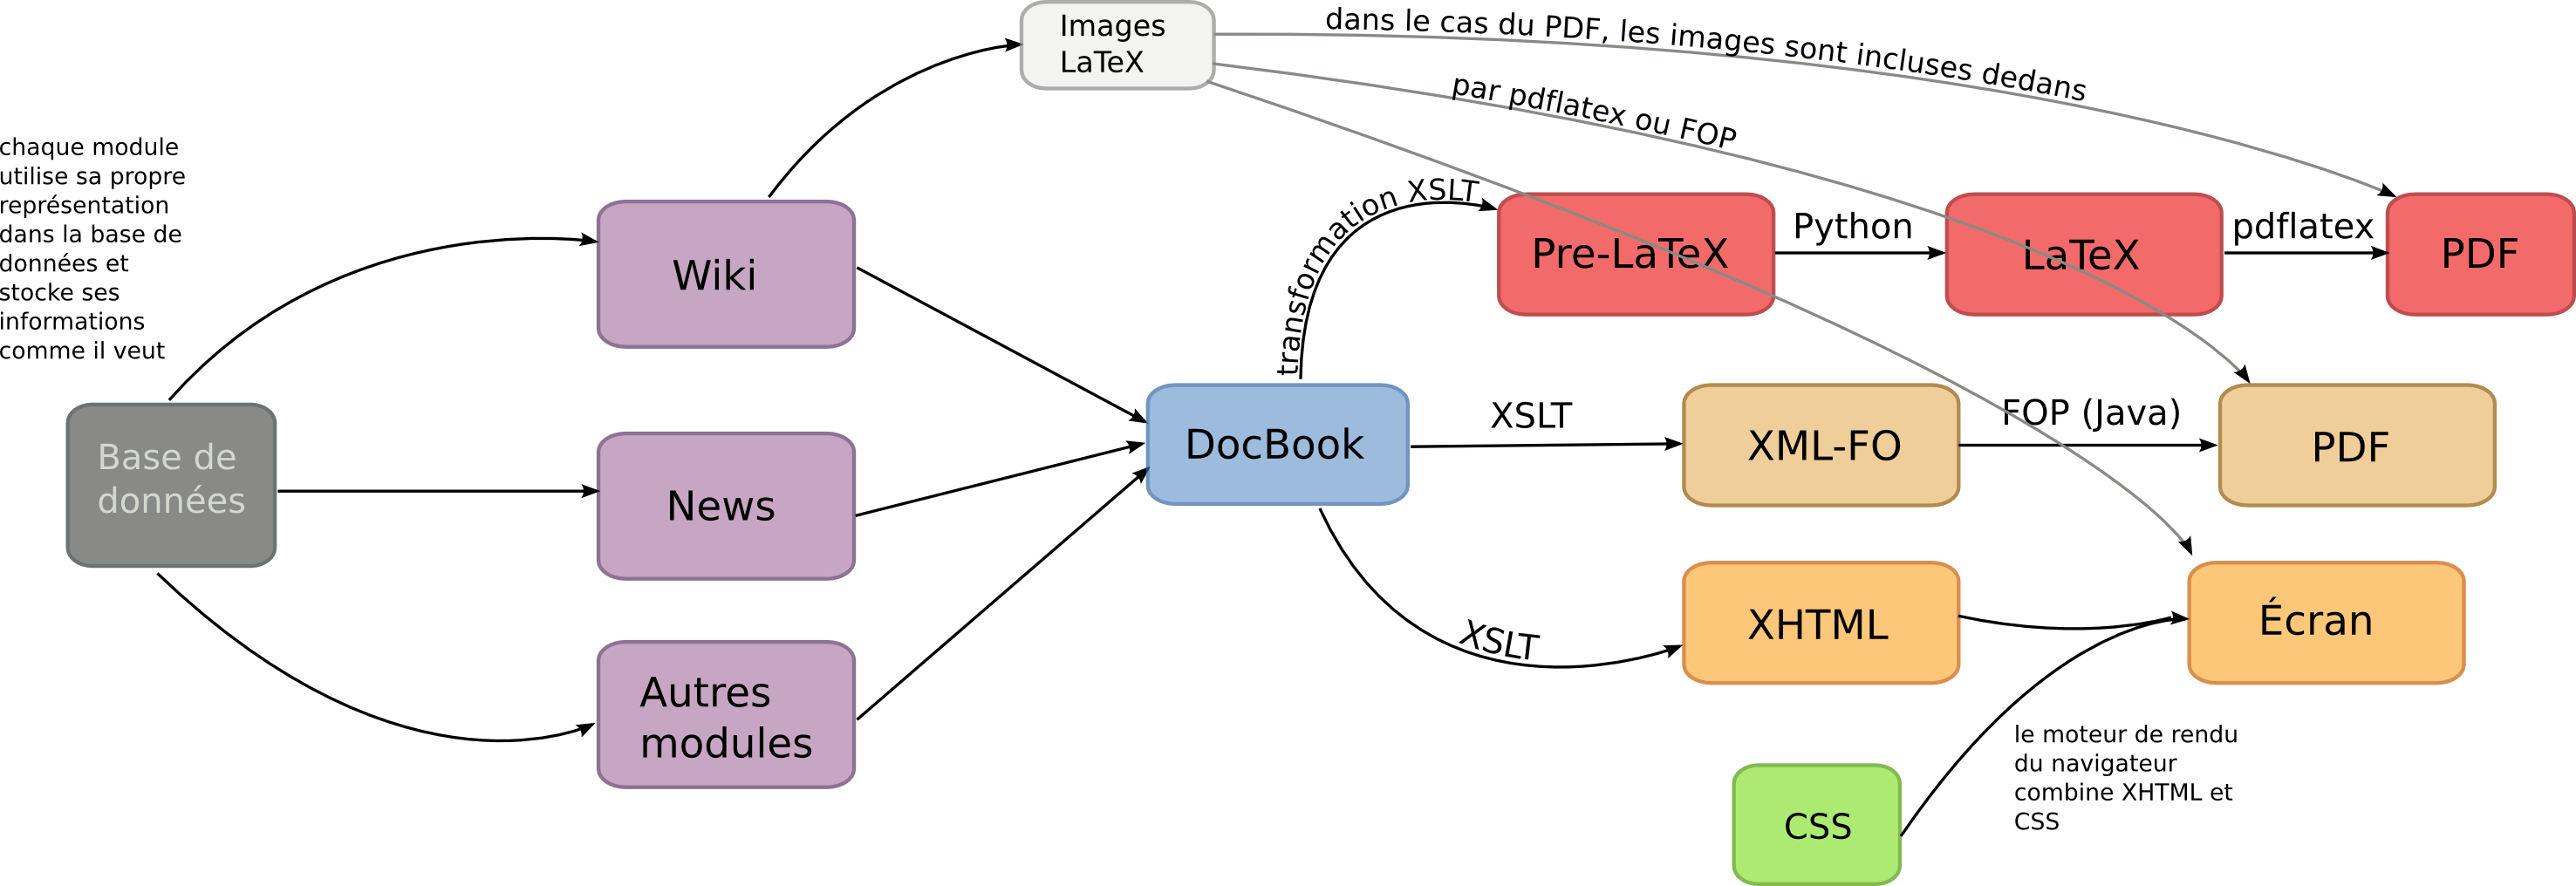
\includegraphics[width=18cm]{drawing.png}
  \end{center}
  \vspace{1em}
  
  \section{La base de données sous-jacente (WP3)}
    \subsection{Avantage des différents types de bases de données}  
  Afin de permettre un bon fonctionnement de l'ensemble des modules, CoMFoRT se devait de 
  contenir une base de données fonctionnelle mais simple. En effet, peu
  nombreuses sont les fonctionnalités spécifiques requises. La tâche la plus complexe 
  demandée à la base de données est un simple select~: la fonction renvoie certains champs 
  précis, en accord avec la condition donnée en entrée. Pour cette raison, et aussi parce 
  que nous pensons qu'elle s'intègre mieux au reste du projet, nous
  avons d'abord voulu privilégier
  une base de données hiérarchique, de type XML. Ce choix permettait une version très légère et
  complètement adaptée de la base de données. \p

  Cependant, nous avons conscience que les bases de données de type relationnel (MySQL, 
  SQLite\ldots) sont aujourd'hui les plus couramment utilisées. Ce sont des systèmes rodés 
  dont les qualités ne sont plus à prouver. Nous avons choisi ce dernier car, contrairement 
  à son grand frère MySQL, il ne 
  nécessite pas l'installation d'un serveur et est directement intégré au programme. Nous 
  pensons implémenter la base de données en MySQL par la suite.\p
  
  La base de données a donc été codée en parallèle en SQLite et en XML. Si la première est
  tout à fait fonctionnelle, la seconde n'est pas totalement terminée mais est sur le point
  d'être intégrée au projet.

    \subsection{API abstraite}
    La gestion des différentes versions n'a pu être possible que par la création d'une API 
    (Application Programming Interface) rigoureuse et entièrement abstraite. Cette dernière 
    définit les fonctions utilisées en gérant les contraintes des différents types de bases 
    de données. Dans le cadre du projet, les fonctions utilisées restent trop limitées pour 
    que le fait d'imposer une API assez abstraite pour rentrer à la fois dans le cadre du 
    hiérarchique et du relationnel soit un problème. Ainsi, l'utilisateur est en mesure 
    d'utiliser la base de données qu'il souhaite de manière totalement flexible et efficace.\p
    
    L'API contient toutes les fonctions basiques nécessaires: ajout,
    suppression de tables, champs,
    verrouillage\ldots \p
    
    Citons comme exemples, dans la classe des tables,
    \code{insert(self, record)} insère le dictionnaire 
    <<~record~>> comme champ dans la table et retourne éventuellement
    son id ou encore ~\code{select(self, order = None, cond = None,
    limit = None, offset = None)} recherche les enregistrements 
    de la table qui satisfont la combinaison de conditions décrite par
    <<~cond~>>, triés par les ordres 
    décrits par <<~order~>>, en limitant éventuellement les résultats. Cette dernière fonction est
    surement le facteur limitant de la flexibilité pour la base de données. En effet, imposer aux
    conditions d'être sous forme de ET ou de OU peut réduire les
    possibilités dans certains cas. \p
    
    L'API complète peut se trouver dans le fichier \code{src/db/db\_interface.py} du SVN.
   


  \section{Choix des technologies}
    \subsection{Lexique~: XML, DocBook, XHTML, XSLT, XML-FO, FOP, CSS, \texttt{dblatex}}
      \begin{description}
        \item[XML] est un métalangage~: il définit la structure d'un document
          et l'ensemble des règles auxquelles ce dernier doit se conformer. Un
          document XML est ainsi formé de \emph{balises} (par exemple
          \code{<article>}) qui doivent être fermées (\code{</article>}). Les
          balises XML comportent des attributs sous la forme \code{<balise
          attr1="val1" attr2="val2">}\ldots de nombreuses autres règles
          constituent le langage XML.

          L'avantage de ce métalangage est qu'on peut traiter un document XML
          de la même façon quel que soit le langage en particulier. Par exemple,
          les \emph{parseurs XML} fonctionnent pour tous les langages XML, par
          exemple~: XHTML, RSS, MathML, SVG, XUL\ldots \p

        \item[DocBook] est un langage XML permettant de décrire le contenu
          \emph{sémantique} d'un document, un peu comme \LaTeX{}~: on décrit le
          type de document (livre, article\ldots) et on imbrique des sections,
          des paragraphes. Il n'y a pas de balise gras ou souligné, mais une
          balise \code{<emphasis>} qui donnera un résultat différent selon le
          medium de sortie utilisée.

          DocBook est un langage largement utilisé dans le monde de l'édition
          professionnelle, car il permet de rédiger facilement et simplement un
          livre, un manuel technique. XSLT (voir ci-dessous) permet ensuite de
          transformer un document DocBook en PDF (voir encore plus bas), ou en
          un format propriétaire (Adobe Illustrator) pour que l'imprimeur puisse
          y apporter les corrections finales. \p

        \item[XHTML] est un langage XML qui offre les mêmes possibilités que le
          HTML, avec la rigueur syntaxique de XML en plus. Il permet de décrire
          la structure sémantique d'une page web en balisant des parties de texte
          à la façon XML~: hyperliens, titres, paragraphes, listes, images, et
          plus encore. \p

        \item[XSLT] ou \emph{eXtensible Stylesheet Language Transformation} est
          un autre langage XML qui permet de décrire la manière de transformer
          un document XML en un autre document (pas nécessairement XML)~: on
          parle de feuille XSLT. Par exemple, une feuille XSLT décrira la
          manière de transformer un document DocBook en un document XHTML.

          XSLT est extrêmement puissant~: il peut par exemple générer
          automatiquement une table des matières. \p

        \item[XML-FO] ou XML-Formatting Object est encore un langage XML. Là où
          DocBook comporte un aspect sémantique, XML-FO est présentationnel~: il
          permet de donner des indications quant à la manière de mettre en page
          le document. XML-FO reste générique~: il faut un logiciel pour
          transformer le XML-FO en un format de sortie~: PS, PDF, RTF, et ainsi
          de suite. C'est le rôle du \emph{FO Processor}. \p

        \item[FOP] Les logiciels permettant de transformer XML-FO en un format
          imprimable, ou sauvegardable, sont pour la plupart commerciaux
          (souvent utilisés dans le monde de l'édition). Il en existe néanmoins
          un libre~: FOP, de la fondation Apache (FO Processor). Écrit en Java,
          nous l'utilisons pour transformer le XML-FO en PDF. \p

        \item[CSS] est un langage (pas XML, le seul ici~!) qui est utilisé
          pour décrire la présentation des pages XHTML. Le but principal est
          de clairement distinguer le fond de la forme. On met donc \emph{toutes}
          les informations de mise en forme dans un fichier associé à un site
          web~: la feuille de style. \p

        \item[\texttt{dblatex}] est un logiciel qui permet de transformer, en
          deux passes, un document DocBook en document \LaTeX{}. 
      \end{description}

    \subsection{Pourquoi DocBook}
      Le but étant de générer un site web, le langage utilisé pour stocker et
      communiquer les données de l'utilisateur doit être le plus proche possible
      de XHTML~; mais en manipuler directement aurait été extrêmement compliqué.
      \p

      Nous avons donc opté pour DocBook, un langage XML très simple, mais
      surtout pour lequel il existe une pléthore d'outils à notre disposition.
      C'est ce qui nous permet de passer si facilement d'un format à l'autre.
      Remarquons aussi qu'il est beaucoup plus aisé de garder une syntaxe
      correcte avec du DocBook qu'avec du XHTML. \p

    \subsection{Pourquoi XHTML 1.0}
      Nous considérons que XHTML 1.1 est un langage voué à l'échec. Pour preuve,
      l'infime minorité de sites utilisant la version 1.1 de XHTML. XHTML 1.0
      est l'évolution naturelle de HTML4~: plus propre, mieux structuré, il est
      le prolongement naturel du HTML. En revanche, les prochaines évolutions,
      et le futur du web se situent, selon nous, dans HTML5.

  \section{Les différentes chaînes de production (WP2)}
    \subsection{XHTML}
      Pour générer du XHTML (voir schéma ci-dessus), nous assemblons d'abord le
      DocBook généré par chaque module. Ensuite, une fois que nous avons créé un
      document DocBook correct, nous effectuons une transformation XSLT
      (feuilles de style XHTML de N. Walsh) pour générer du XHTML directement.
      C'est la chaîne de production la plus directe et la plus rapide de
      toutes~: c'est une application directe de la philosophie DocBookienne.

      Il est à noter que le XHTML généré est de fait correct~: toutes les pages
      générées par CoMFoRT sont compatibles XHTML 1.0 transitional.

    \subsection{PDF via FOP}
      La chaîne de production DocBook a été conçue pour prendre en charge une
      immense variété de formats de sortie~: ODT (pour OpenOffice.org 2.0 par
      exemple), RTF, PS et PDF. Pour ce faire, nous utilisons comme
      intermédiaire FO. FO, pour Formatting Object, permet, rappelons le,
      d'exprimer l'aspect présentationnel d'un document à l'aide d'XML. FO donne
      des indications sur la manière de mettre en page le document,
      contrairement à DocBook, qui n'a qu'un contenu sémantique. \p

      Une fois le fichier XML-FO généré, il faut un logiciel de mise en page
      pour transformer FO en un format de sortie. Plusieurs logiciels
      commerciaux sont disponibles sur le marché (témoignant ainsi de la
      présence de DocBook dans le monde de l'impression et de l'édition)~; un
      logiciel libre l'est également~: FOP, pour FO Processor. Projet de la
      fondation Apache, il est écrit en Java. \p

      Il suffit donc de lance FOP sur le fichier XML-FO produit précédemment, en
      indiquant PDF comme format de sortie~: le PDF est généré.

    \subsection{PDF via \LaTeX}
      Cependant, FOP, projet libre, n'atteint pas la qualité d'un logiciel de
      mise en page professionnel. Quel est le logiciel libre permettant de
      produire des documents d'une qualité professionnelle~? \LaTeX{} bien sûr~!
      Nous avons donc mis en place une seconde chaîne de production pour le
      format PDF. Ceci est possible grâce au projet dblatex, qui se charge
      justement d'effectuer cette tâche. \p

      Une feuille XSLT effectue le gros de la transformation vers \LaTeX{}. Les
      quelques incorrections restantes\footnote{Se référer au site de dblatex
      pour plus de précisions.} sont corrigées à l'aide d'un dernier passage en
      Python. On peut alors lancer \code{pdflatex} sur le fichier \code{.tex}
      obtenu pour obtenir un PDF de bien meilleure qualité.

  \section{Les styles (WP2)}
    La gestion de styles se fait à partir de feuilles CSS uniquement. Le code
    XHTML des pages ne contient pas de mise en forme et est invariant par
    changement de thème. Inversement, les feuilles de style ne varient pas en
    fonction du contenu de la page~: à chaque style correspond une feuille CSS
    qui contient les informations sur les tous les éléments possibles d'un
    site web créé avec CoMFoRT.

    \subsection{Les différentes catégories de styles}
      Nous avons dégagé plusieurs catégories de styles.
      \begin{description}
        \item[Les styles officiels] sont des styles que nous considérons
          suffisamment aboutis~: ce sont les styles de meilleure qualité. Nous
          nous engageons à les maintenir au fil du temps et à garantir toujours
          leur parfaite adaptation au CMS. Il est à noter que tous ces styles
          sont validés par jigsaw, le validateur CSS du W3C.
        \item[Les styles semi-officiels] sont des styles qui, ou bien parce
          qu'ils font appel à du CSS3 (pas encore bien implémenté partout)
          comme <<~TheManor~>>, ou bien parce qu'ils sont plus fantaisistes
          (comme <<~TheManor~>>), sont moins mis en avant que les styles
          officiels. Ils bénéficient quand même d'un minimum d'attention, et
          sont a priori des styles que nous visons à améliorer pour en faire
          des styles officiels (<<~GreenyGrass~>> par exemple).
        \item[Les autres catégories] sont pour des styles qui sont disponibles
          en plusieurs couleurs (style <<~Twisted~>>).
        \item[Les autres styles] sont des styles que nous considérons de
          mauvaise qualité et que nous n'incluons pas pour cette raison dans
          les catégories ci-dessus. Certains sont l'\oe{}uvre d'un jour,
          d'autres sont juste des essais. Nous les laissons en espérant qu'une
          âme charitable leur donnera un peu d'attention pour les faire passer
          dans une autre catégorie.
      \end{description}
  \section{Serveur, synchronisation et génération (WP6)}
    Une fois le site créé, reste encore à le mettre en ligne. Pour cela, il suffit
    à l'utilisateur de se rendre dans la section <<~Synchronisation~>> de l'interface
    d'administration, d'y choisir une synchronisation par FTP, par SSH ou bien encore
    simple génération d'une archive contenant tout le site, d'y entrer les informations
    nécessaires en fonction de ce choix puis d'y cliquer sur le bouton Synchroniser
    pour qu'automatiquement la version statique du site soit générée et envoyée sur le
    serveur distant et ainsi disponible au monde entier.

    \subsection{Fonctionnalités}
    \begin{itemize}
    \item Support de différents modes de synchronisation~: FTP, SSH (non encore
      pleinement fonctionnel), génération d'une archive (à implémenter).
    \item Envoi uniquement des fichiers modifiés (et oui c'est même utilisable pendant
      votre conf' au fin fond du désert de Gobi avec une antique connexion 56k).
    \item Possibilité de modifier le site sur plusieurs machines, la synchronisation
      effectue également une réception des fichiers qui ont été modifiés sur le serveur.
      Ainsi le site peut être créé sur une machine $A$, synchronisé (envoi), resynchronisé
      sur une machine $B$ (réception de ce qui a été fait sur la machine $A$), modifié,
      resynchronisé (envoi des modifications) puis resynchronisé si un jour on revient
      sur la machine $A$ (récupération des modifications faites sur $B$).
    \end{itemize}

    \subsection{Problèmes rencontrés}
    La base de données étant monolithique, toute modification qui serait faite sur la machine $A$
    (cf. ci-dessus) avant de resynchroniser les modifications faites sur $B$ entraînerait
    immédiatement un conflit même si ces modifications n'ont aucun
    rapport avec celles faites sur $B$.
    Avantage ici de la base de données XML~: on pourrait tenter
    d'appliquer les techniques de merge
    développées pour les systèmes de gestion de versions.


\part{Contribuer}
  \section{Améliorations prévues}
    Les différentes remarques qui nous ont été faites sont en cours
    d'intégration~: nous espérons sortir une version définitive à la rentrée
    2008.
    \begin{description}
      \item[L'importation/exportation] du site depuis/dans un fichier précis
        pour sauvegarder son site (compatible avec chaque version de CoMFoRT)
      \item[Le module menu] devrait être amélioré pour prendre en compte des
        catégories d'items.
      \item[La localisation] devrait être \emph{vraiment} faite avec la
        possibilité de rentrer chaque contenu en double pour générer
        automatiquement un site dans chaque langue.
      \item[Une balise <module>] mieux exploitée et plus facile à utiliser
      \item[Une gestion des mises à jour]: proposer un lien quand il existe une
        nouvelle version de CoMFoRT
      \item[De nouveaux thèmes] pour CoMFoRT: clairs et sérieux     
      \item[D'autres améliorations] sont prévues sur
        \url{http://graal.ens-lyon.fr/confort/wiki/TODO}. 
    \end{description}

  \section{Créer un style}
    Rien de plus simple~! Il suffit de créer un dossier sous la forme
    \code{nomdustyle} dans le dossier \code{styles}~: <<~nomdustyle~>>
    apparaîtra automatiquement dans l'administration. Ce dossier doit contenir
    un fichier \code{style.css}. Ce dernier doit inclure le fichier
    \code{wiki.css} situé dans le dossier \code{common} afin d'offrir la mise en
    forme basique du wiki (souligné, surligné, barré\ldots).

    À noter que vous pouvez également créer dans le dossier de votre style un
    fichier \code{latex.dat} qui contient deux lignes. La première contient la
    couleur de fond pour les images \LaTeX{} et la seconde la couleur du texte
    dans les images \LaTeX{}. Les deux couleurs sont au format HTML
    \code{\#rrggbb}. Si ce fichier n'est pas inclus, les images seront avec du
    texte noir sur fond transparent.

    Les styles <<~blue~>> et <<~lite~>> sont largement commentés et
    contiennent tous les sélecteurs dont vous pourriez avoir besoin.
    N'hésitez pas à utiliser l'excellente extension de Firefox~: Firebug
    pour inspecter le document XHTML~: voir quel est l'élément qui déborde,
    pourquoi tel ou tel bloc n'est pas correctement aligné, et ainsi de
    suite.



  \section{Créer un module}
    Pour créer un module, il suffit de créer un fichier
    \code{themodule\_NomDuModule.py} dans le dossier \code{modules}, et d'écrire
    une classe \code{TheModule} qui implémente impérativement
    \code{IComfortModule}. La classe pourra éventuellement implémenter d'autres
    interfaces selon les fonctionnalités qu'elle vise. Ne pas hésiter à nous
    contacter pour obtenir des informations plus précises sur les interfaces
    futures et existantes.

    Le module aura probablement à gérer une interface d'administration. Pour
    cela, regardez le module <<~Crédits~>>~: il est très simple, et permet de
    comprendre rapidement comment gérer une page d'administration.

    Pour voir comment récupérer les résultats d'un formulaire d'administration,
    vous pouvez par exemple consulter le module <<~Coordonnées~>>. Ce dernier
    vous apprendra également comment travailler avec la base de données.

    Si vous avez besoin de fonctionnalités plus évoluées (par exemple accéder à
    un autre module), vous pouvez récupérer l'instance du ModuleManager grâce
    à~:
    \begin{verbatim}
      from modules import module_manager
      mm = module_manager.ModuleManager()
    \end{verbatim}
    Le design pattern Singleton
    (\url{http://en.wikipedia.org/wiki/Singleton_pattern}) garantit que vous
    récupérez bien l'instance qui sert à générer la page en cours.

  \section{Où trouver de la documentation}
    La documentation générée en ligne (voir dossier \code{doc}) dans le SVN vous
    permet de lire plus facilement tous nos commentaires. Des diagrammes de
    classe sont aussi générés et vous permettent de voir, pour les différents
    modules, les interfaces qu'ils implémentent.

    De la documentation est également présente dans le dossier \code{doc}, et le
    wiki du projet contient aussi des informations précieuses. Encore une fois,
    n'hésitez pas à nous contacter sur la mailing-list (pour l'instant~:
    \url{projet2@listes.ens-lyon.fr}) pour nous faire part de vos
    interrogations.
\end{document}
